\section{Results}
\label{sec:results}
\label{sec:frontier}
\label{sec:openweight}

% Verdict table (code_council/build_verdicts.py); needs numbers_c_verdicts.tex.
% The like-for-like column is from code_council/peer_discrimination.py (p_dd, Holm within setting).
\begin{table}[t]
\centering\small
\begin{adjustbox}{max width=\linewidth}
\begin{tabular}{lllll}
\toprule
& & & \multicolumn{2}{c}{Also exceeds peers} \\
\cmidrule(lr){4-5}
Judges, texts, format & Self-naming above chance & Also discriminates & Raw baseline & Like-for-like \\
\midrule
Frontier, chat-app essays, lineup & GPT, Claude & GPT, Claude & GPT, Claude & GPT, Claude \\
Frontier, chat-app essays, one text & GPT, Claude & GPT, Claude & GPT & GPT, Claude \\
Frontier, chat-app essays, yes/no & Claude & Claude & n/a & n/a \\
Frontier, API texts, lineup & Claude, Grok & Claude, Grok & -- & -- \\
Frontier, API texts, one text & GPT, Claude & Claude & -- & Claude \\
Open-weight, lineup & Qwen & -- & -- & -- \\
Open-weight, one text & Qwen, Llama, Phi & -- & -- & -- \\
Open-weight, yes/no & Llama, Mistral & -- & n/a & n/a \\
\midrule
Cases & \CVflagged{} of \CVcells{} & \CVdisc{} of \CVcells{} & \CVbothAttr{} of \CVattr{} & \CXLikeForLike{} of \CVattr{} \\
\bottomrule
\end{tabular}
\end{adjustbox}
\caption{Which judges are flagged by the self-naming test, and which of them
pass each control (definitions in Section~\ref{sec:setup}). The columns are
nested from left to right; the last two give the peer control in two forms.
\emph{Raw baseline}: the judge names itself on its texts more often than the
other judges name it. \emph{Like-for-like}: the judge's discrimination exceeds
the mean discrimination of the other judges for the same author, which removes
each peer's general tendency to name that model. The yes/no format has no peer
baseline (n/a), so the last two columns count only the \CVattr{} lineup and
one-text cases. Claude on the chat-app essays is the only yes/no case that
discriminates, and it does so only with correction within the panel
($p=$~\FBClaudeHolm{}; $p=\CXClaudeYesNoHolmAll$ across all \CVcells{} cases).
All tests are Holm-corrected across the judges of a panel.}
\label{tab:verdicts}
\end{table}


\paragraph{The self-naming test and the two controls}
Table~\ref{tab:verdicts} applies the self-naming test and both controls to
every case. The self-naming test flags \CVflagged{} of the \CVcells{} cases.
In \CVfailFA{} of them the judge names itself about as often on texts it did
not write as on its own: \CVopenFlagged{} open-weight cases, and GPT on the API
texts shown one at a time. The other \CVdisc{} discriminate. \CVbothAttr{} of
these also exceed their peer baseline, and one, Claude in the yes/no format,
has no peer baseline. The remaining \CVfailPeer{}, Claude in three settings and
Grok in one, discriminate by \FXGrokLineupDisc{} to \CXClaudeChatSingleDisc{}
points without exceeding their peers. These judges can tell their own texts
from others', so anonymisation offers them limited protection; what they lack
is an advantage over the other judges. Figure~\ref{fig:verdictmap} shows that
the two kinds of failure lie along different axes. Of the \CVflaggedAttr{}
flagged cases that have a peer baseline, \CVpeerSurvive{} pass it, so the
false-alarm control removes most cases overall, and the peer baseline removes
most of those among the frontier judges (4 of 5). Every case that
discriminates is also flagged. By panel, the self-naming test flags
\CVfrontierFlagged{} of the \CVfrontierCells{} frontier cases, of which
\CVfrontierDisc{} discriminate, and \CVopenFlagged{} of the \CVopenCells{}
open-weight cases, of which none does. In \CXFixedCells{} cases the judge gives
the same answer on at least 97\% of texts; among the other \CXVaryCells{} the
three counts are \CXVaryFlagged{}, \CVdisc{} and \CVbothAttr{}
(Appendix~\ref{app:stats}).

\begin{figure}[t]
\centering
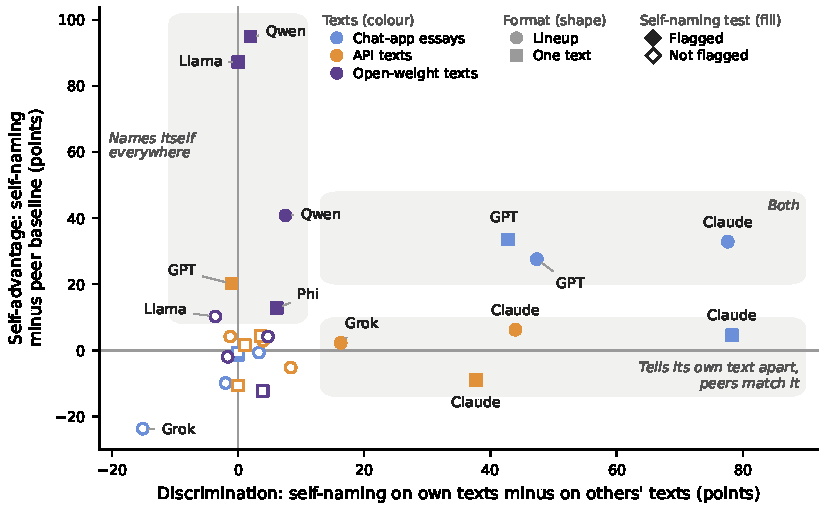
\includegraphics[width=0.85\linewidth]{figures/verdict_map.pdf}
\caption{The \CVattr{} lineup and one-text cases, placed by discrimination
(horizontal) and self-advantage (vertical). Colour gives the text set, shape
the format, and filled markers are the \CVflaggedAttr{} cases flagged by the
self-naming test. The yes/no cases are omitted because they have no peer
baseline. Flagged cases near the vertical axis exceed their peers, by up to
\OWQwenSingleAdv{} points, without discriminating; those near the horizontal
axis discriminate while their peers name them about as often; three are far
from both axes. The grey bands are reading guides; the verdicts come from the
tests in Table~\ref{tab:verdicts}.}
\label{fig:verdictmap}
\end{figure}

\begin{figure}[t]
\centering
\begin{subfigure}[b]{\linewidth}\centering
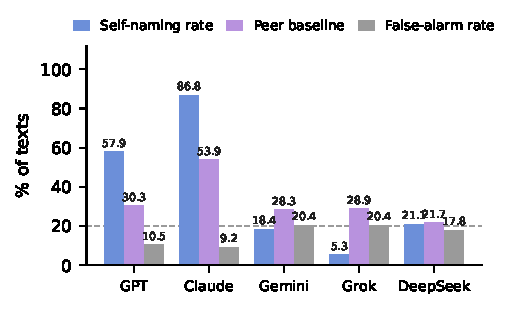
\includegraphics[width=\linewidth]{figures/lead_lineup.pdf}
\caption{Lineup}\label{fig:lead-lineup}
\end{subfigure}

\vspace{4pt}
\begin{subfigure}[b]{\linewidth}\centering
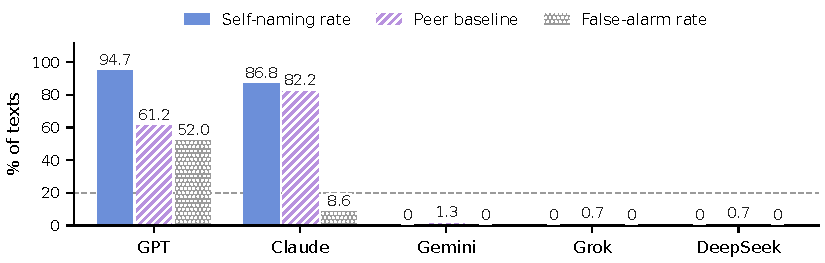
\includegraphics[width=\linewidth]{figures/lead_single.pdf}
\caption{One text at a time}\label{fig:lead-single}
\end{subfigure}
\caption{Self-naming rate, peer baseline and false-alarm rate of the five
frontier judges on the 38 chat-app essays each wrote. The self-naming rate is
the share of its own essays a judge attributes to itself, the peer baseline is
the share of those essays the other four judges attribute to it, and the
false-alarm rate is the share of other models' essays it attributes to itself.
In the lineup (a), Claude and GPT exceed their peer baselines by 33 and 28
points and Grok falls 24 points below its baseline. When the same essays are
shown one at a time (b), Gemini, Grok and DeepSeek never name themselves, GPT
names itself on 52\% of essays it did not write, and Claude's peer baseline
rises to 82\%. The dashed line marks chance (20\%).}
\label{fig:lead}
\end{figure}

\begin{table}[t]
\centering\small\setlength\tabcolsep{3.5pt}
\begin{adjustbox}{max width=\linewidth}
\begin{tabular}{llrrrrrr}
\toprule
Format & Judge & Self-naming & False alarms & Peer baseline & Self-adv. [95\% CI] & $p$ (Holm) & Skill-adj. \\
\midrule
Lineup & GPT & 22/38 & 16/152 & 46/152 & +27.6 [+10.5, +44.7] & $0.008$ & +19.3 \\
 & Claude & 33/38 & 14/152 & 82/152 & +32.9 [+21.1, +44.1] & $0.002$ & +35.1 \\
 & Gemini & 7/38 & 31/152 & 43/152 & $-$9.9 [$-$23.0, +4.6] & $0.619$ & $-$19.3 \\
 & Grok & 2/38 & 31/152 & 44/152 & $-$23.7 [$-$32.9, $-$13.2] & $0.008$ & $-$20.2 \\
 & DeepSeek & 8/38 & 27/152 & 33/152 & $-$0.7 [$-$15.1, +15.1] & $1.000$ & +11.4 \\
\midrule
Single & GPT & 36/38 & 79/152 & 93/152 & +33.6 [+25.0, +42.1] & $2.1\times10^{-4}$ & -- \\
 & Claude & 33/38 & 13/152 & 125/152 & +4.6 [$-$7.2, +14.5] & $1.000$ & -- \\
 & Gemini & 0/38 & 0/152 & 2/152 & $-$1.3 [$-$3.3, +0.0] & $1.000$ & -- \\
 & Grok & 0/38 & 0/152 & 1/152 & $-$0.7 [$-$2.0, +0.0] & $1.000$ & -- \\
 & DeepSeek & 0/38 & 0/152 & 1/152 & $-$0.7 [$-$2.0, +0.0] & $1.000$ & -- \\
\bottomrule
\end{tabular}
\end{adjustbox}
\caption{Frontier judges on the chat-app essays. Self-naming: the judge names itself on its own 38 texts. False alarms: it names itself on the 152 texts it did not write. Peer baseline: the other four judges name it on its texts. Self-advantage is the difference in rates, with a prompt-bootstrap interval; $p$ is the exact within-response randomisation test, Holm-corrected over the five judges. Skill-adjusted removes each judge's general accuracy and each author's identifiability (Appendix~\ref{app:stats}); it is not interpretable in single-text, where a judge's accuracy mostly reflects which model it habitually names. In single-text, Gemini, Grok and DeepSeek never name themselves.}
\label{tab:frontier}
\end{table}


\paragraph{Lineup format, chat-app essays}
Claude names itself on 33 of its 38 essays (87\%) and on 14 of the 152 essays it
did not write (9\%); the other judges name Claude on 54\% of Claude's essays
(Table~\ref{tab:frontier}, Figure~\ref{fig:lead-lineup}). Claude's
self-advantage is \ClaudeAdvLineup{} points \ClaudeAdvLineupCI{} and GPT's is
\GPTAdvLineup{} \GPTAdvLineupCI{}. Both judges have false-alarm rates near
10\% and discriminate. In this format the discrimination test adds little to
the self-naming test, because the frontier judges use each of the five names
once in \CROneToOneChat{} of lineups (Appendix~\ref{app:stats}); the peer
baseline is the control that separates the two here. The peers are unequal
(Figure~\ref{fig:naming}a). GPT names Claude on \CRGPTOnClaudeHitK{} of
Claude's 38 essays (\CRGPTOnClaudeHit{}) and on \CRGPTOnClaudeFAK{} of the 152
other essays, which matches Claude's own rates, whereas Grok and DeepSeek each
name Claude on \CRGrokOnClaudeHit{} of Claude's essays. Claude's self-advantage
is therefore an advantage over the average peer; over GPT alone the difference
is \CRClaudeVsBestPeer{} points \CRClaudeVsBestPeerCI{}. GPT names itself more
often than each individual peer names it (\GPTSelfLineup{} against
\CRPeersOnGPTMin{} to \CRPeersOnGPTMax{}). DeepSeek and Gemini have no significant
self-advantage. Grok names itself on 2 of its 38 essays, and its self-advantage
is significantly negative (\GrokAdvLineup{} \GrokAdvLineupCI{}). The results
for Claude, GPT and Grok are unchanged in mixed-effects models and after
adjusting for each judge's overall attribution accuracy
(Appendix~\ref{app:stats}). They are also unchanged when the self-advantage is
computed within each position of the lineup and averaged (Table~\ref{tab:anchor}).

\begin{figure}[t]
\centering
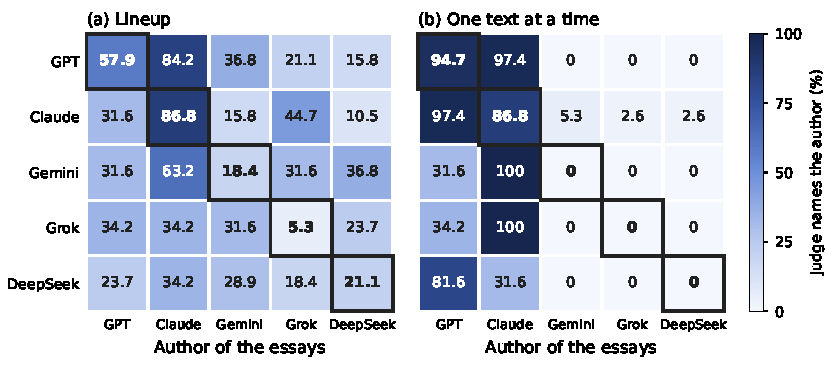
\includegraphics[width=\linewidth]{figures/naming_matrix.pdf}
\caption{How often each frontier judge (row) names the true author (column)
on that author's 38 chat-app essays, in percent, (a) in the lineup and (b) one
text at a time. Outlined cells on the diagonal are self-naming rates, and the
mean of the other four cells in a column is that author's peer baseline.}
\label{fig:naming}
\end{figure}

\paragraph{One-text format, chat-app essays}
When essays are shown one at a time, \SingleConcentration{} of attributions name
GPT or Claude (Figure~\ref{fig:guess} in Appendix~\ref{app:more}), as in \citet{bai2025selfrecognition}.
Gemini, Grok and DeepSeek never name themselves, so this format provides no
useful measure of discrimination for these judges. GPT's self-naming rate
rises to \GPTSelfSingle{}, and its false-alarm rate to 52\%. Claude's
self-naming rate stays at \ClaudeSelfSingle{}, but its peer baseline rises to
\ClaudePeerSingle{}, and its self-advantage falls to \ClaudeAdvSingle{} points
(Figure~\ref{fig:lead-single}). Claude's discrimination is almost the same as
in the lineup (\CXClaudeChatSingleDisc{} points), so the lower self-advantage
comes from its peers, mainly from Gemini and Grok, which name Claude on all 38 of Claude's
essays and also on \CRGeminiOnClaudeSingleFA{} and \CRGrokOnClaudeSingleFA{} of
the essays Claude did not write (Table~\ref{tab:naming}). The peer baseline
thus includes the peers' general tendency to name a model, and it is
informative only when judges distribute their attributions across models.
A like-for-like comparison, the judge's discrimination minus the mean
discrimination of its peers for the same author, removes this tendency from
both sides. Under it, five of the \CVattr{} lineup and one-text cases exceed
their peers after Holm correction: Claude and GPT in both formats on the
chat-app essays, and Claude one text at a time on the API texts ($+20.5$
points $[+12.5, +28.6]$). Claude's one-text margin on the chat-app essays is
$+51.3$ points $[+38.6, +62.8]$ under this comparison, against
\ClaudeAdvSingle{} on raw rates. Table~\ref{tab:verdicts} reports both forms.
The raw baseline is the simpler quantity and the one a lineup gives directly;
the like-for-like form is the fairer comparison when peers differ in how often
they name a model, and it adds the two Claude one-text cases. GPT
passes both controls in this format, but Claude names GPT on 37 of GPT's 38
essays, about as often as GPT does, and GPT names itself on 34 of Gemini's 38
essays; its self-advantage arises because Gemini and Grok name GPT on only 12
and 13 of its essays (Figure~\ref{fig:naming}b).

\paragraph{Yes/no format, chat-app essays}
GPT, Grok and DeepSeek answer no for all 190 essays, including their own 38
(Figure~\ref{fig:yes-frontier} in Appendix~\ref{app:more}), although all three name themselves in the
lineup. Gemini answers yes twice, both times for essays it did not write. Claude
answers yes for \FBClaudeHitK{} of its own essays and \FBClaudeFAK{} of other
models' essays, a discrimination of \FBClaudeDisc{} points (Holm
$p=$~\FBClaudeHolm{}). This is the weakest of the \CVdisc{} cases that
discriminate: the bootstrap interval for its discrimination is
\CXClaudeYesNoDiscCI{}, and the result is not significant when corrected
across all \CVcells{} cases ($p=\CXClaudeYesNoHolmAll$). GPT, which names
itself on 95\% of its own essays in the one-text format, does not claim any of
them in this format. These uniform answers are hard to interpret. The question
is asked in a new conversation, and \CXReasonGPTBroad{} of the
\CXReasonGPTN{} reasoning summaries returned for GPT and \CXReasonGrokBroad{}
of Grok's 190 state that the judge has no memory of writing the text or cannot
verify its authorship (Appendix~\ref{app:rationales}). We therefore draw no
conclusion from these answers about whether GPT and Grok can recognise their
own style, and we have no such information for DeepSeek.

\begin{table}[t]
\centering\small
\setlength\tabcolsep{2.5pt}
\begin{adjustbox}{max width=\linewidth}
\begin{tabular}{l rrr rr}
\toprule
Judge & Self & Peer & FA & Self-adv. [95\% CI] & Hit$-$FA \\
\midrule
\multicolumn{6}{l}{\emph{Lineup}} \\
GPT & 19.2\% & 15.0\% & 20.4\% & +4.2 [$-$3.3, +12.1] & $-$1.2 \\
Claude & 56.7\% & 50.4\% & 12.7\% & +6.2 [$-$2.5, +14.8] & +44.0$^{*}$ \\
Gemini & 26.7\% & 31.9\% & 18.3\% & $-$5.2 [$-$14.4, +3.8] & +8.3 \\
Grok & 32.5\% & 30.2\% & 16.2\% & +2.3 [$-$7.1, +11.9] & +16.2$^{*}$ \\
DeepSeek & 21.7\% & 18.8\% & 17.7\% & +2.9 [$-$5.2, +11.5] & +4.0 \\
\midrule
\multicolumn{6}{l}{\emph{One text at a time}} \\
GPT & 83.3\% & 63.1\% & 84.4\% & +20.2$^{*}$ [+13.5, +26.7] & $-$1.0 \\
Claude & 40.8\% & 49.8\% & 3.1\% & $-$9.0 [$-$16.0, $-$1.5] & +37.7$^{*}$ \\
Gemini & 8.3\% & 4.0\% & 4.8\% & +4.4 [$-$0.4, +9.6] & +3.5 \\
Grok & 1.7\% & 0.0\% & 0.6\% & +1.7 [+0.0, +4.2] & +1.0 \\
DeepSeek & 0.0\% & 10.6\% & 0.0\% & $-$10.6$^{*}$ [$-$12.9, $-$8.3] & +0.0 \\
\bottomrule
\end{tabular}
\end{adjustbox}
\caption{The five frontier judges on 600 texts the same five models wrote through the API for 120 prompts in four genres (120 own texts per judge). Columns as in Table~\ref{tab:frontier}; $^{*}$Holm-corrected within-prompt permutation $p<0.05$.}
\label{tab:frontier120}
\end{table}


\paragraph{Lineup and one-text formats, API texts}
On the 600 API texts, no judge has a significant self-advantage in the lineup
(Table~\ref{tab:frontier120}). Claude still discriminates, naming itself on
\FXClaudeLineupSelf{} of its own texts and \FXClaudeLineupFA{} of other models'
texts, but its peers name Claude on \FXClaudeLineupPeer{} of its texts, and
Gemini does so on \CRGeminiOnClaudeApiHit{}, more often than Claude itself.
Grok also discriminates on these texts (\FXGrokLineupDisc{} points), although
its self-advantage on the chat-app essays was negative. Shown one text at a
time, Claude again discriminates (\FXClaudeSingleDisc{} points) and its
self-advantage is negative. Claude's discrimination is largest on essays and
near zero on math problems, where answers to the same problem share most of
their wording (Appendix~\ref{app:more}).

The direct comparison with the chat-app essays uses the \CSprompts{} essay
prompts that the two sets share (Figure~\ref{fig:shared};
Table~\ref{tab:shared}). There the self-advantages of Claude and GPT are about
half as large (\FXOldClaudeLineupAdv{} and \FXOldGPTLineupAdv{} points) and not
significant after correction. The two judges differ in what changed. Claude
names itself on \CSClaudeAPISelfK{} of its 38 API essays, compared with
\CSClaudeChatSelfK{} of its 38 chat-app essays, and its discrimination is
\CSClaudeAPIDisc{} points compared with \CSClaudeChatDisc{}. Its self-advantage
is smaller because its peers name it more often, on \CSClaudeAPIPeer{} of its
API essays compared with \CSClaudeChatPeer{} of its chat-app essays. GPT names
itself on \CSGPTAPISelfK{} of its 38 API essays, compared with
\CSGPTChatSelfK{}, and its discrimination falls from \CSGPTChatDisc{} to
\CSGPTAPIDisc{} points (difference \CSGPTDiscDiff{}, 95\% bootstrap interval
over prompts \CSGPTDiscDiffCI{}). For both judges the difference in
self-advantage between the two text sets is \CSClaudeAdvDiff{} points, and both
intervals include zero (\CSClaudeAdvDiffCI{} for Claude, \CSGPTAdvDiffCI{} for
GPT). The API texts therefore give weaker evidence for GPT, whose
discrimination declines, and are inconclusive for Claude, whose smaller
self-advantage is statistically compatible with its chat-app value. For GPT,
Grok and DeepSeek the chat-app essays were written under a different product
label from the API texts (Section~\ref{sec:setup}), so a change of writer
cannot be excluded as a cause of the difference.

\begin{figure}[t]
\centering
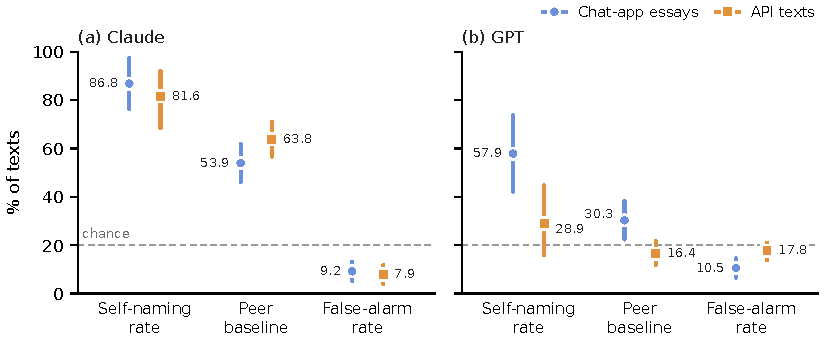
\includegraphics[width=0.85\linewidth]{figures/shared38.pdf}
\caption{Claude and GPT in the lineup on the \CSprompts{} prompts shared by
the chat-app essays (circles) and the API texts (squares): self-naming rate,
peer baseline and false-alarm rate, with 95\% bootstrap intervals over
prompts. Claude's self-naming and false-alarm rates are almost the same on the
two sets and its peer baseline is higher on the API texts; GPT's self-naming
rate and peer baseline fall and its false-alarm rate rises. The dashed line
marks chance (20\%).}
\label{fig:shared}
\end{figure}

\begin{table*}[t]
\centering\small
\setlength\tabcolsep{3.5pt}
\begin{tabular}{l rrrrr rrr rr}
\toprule
 & \multicolumn{5}{c}{Lineup} & \multicolumn{3}{c}{Yes/no, fresh context} & \multicolumn{2}{c}{Own likelihood} \\
\cmidrule(lr){2-6}\cmidrule(lr){7-9}\cmidrule(lr){10-11}
Judge & Self & Peer & FA & Self-adv. [95\% CI] & Hit$-$FA & Hit & FA & AUC & Pick-self & AUC \\
\midrule
Qwen & 56.7\% & 15.8\% & 49.2\% & +40.8$^{*}$ [+31.1, +50.6] & +7.5 & 51.7\% & 58.6\% & 0.45 & 100.0\% & 1.00 \\
Llama & 32.5\% & 22.2\% & 36.1\% & +10.3$^{*}$ [+1.9, +18.6] & $-$3.6 & 85.8\% & 85.6\% & 0.53 & 100.0\% & 1.00 \\
Mistral & 25.0\% & 20.8\% & 20.3\% & +4.2 [$-$6.1, +14.4] & +4.7 & 99.2\% & 99.4\% & 0.41$^{*}$ & 100.0\% & 1.00 \\
Phi & 20.8\% & 22.8\% & 22.5\% & $-$1.9 [$-$10.6, +6.9] & $-$1.7 & 4.2\% & 1.4\% & 0.53 & 100.0\% & 1.00 \\
\bottomrule
\end{tabular}
\caption{Open-weight judges, all four genres pooled (120 prompts). Lineup: self-naming, peer-baseline and false-alarm (FA) rates, the self-advantage with a prompt-bootstrap interval, and the hit minus false-alarm rate, which is positive only if a judge names itself more on its own text than on others'. Yes/no: ``Did you write this text?'' in a fresh context; hit and false-alarm rates at $P(\text{yes})>0.5$ and the AUC of $P(\text{yes})$ for own versus others' text (0.5 is chance). Own likelihood: the share of prompts on which the text the judge finds most likely, relative to the other judges, is its own (chance 25\%), and the AUC of that relative likelihood. $^{*}$Holm-corrected within-prompt permutation $p<0.05$ across the four judges.}
\label{tab:openweight}
\end{table*}


\paragraph{Open-weight judges}
No open-weight judge recognises itself in the lineup
(Table~\ref{tab:openweight}). Qwen and Llama have significant self-advantages
but do not discriminate. Qwen names itself on \OWQwenLineupSelf{} of its own
texts and \OWQwenLineupFA{} of other models' texts, and Llama names itself more
often on other models' texts than on its own. The lineup answers of these
judges depend mainly on the position of a response: the name a judge gives
most often in each position reproduces \CXSlotShare{} of the 1,920
attributions (from \CXSlotShareMin{} for Qwen to \CXSlotShareMax{} for Phi;
Appendix~\ref{app:openweight}). The self-advantages of Qwen and Llama
therefore reflect preferences for a name and a position that these judges
apply to all texts. In the one-text format, Qwen names itself on
\OWQwenSingleNamesSelf{} of all texts and Llama on all of them, the
over-attribution described by \citet{bai2025selfrecognition}. In the yes/no
format, Mistral answers yes for \OWMistralBinaryHit{} of its own texts and
\OWMistralBinaryFA{} of others, and Phi for \OWPhiBinaryHit{} and
\OWPhiBinaryFA{} (Table~\ref{tab:openweight}). The AUC, which does not depend
on a judge's overall rate of yes answers, lies between 0.41 and 0.53 for all
four judges. Overall lineup accuracy is \OWLineupAcc{} (chance 25\%), while the
style classifier attributes \OWClfPooled{} of the same texts. In this panel the
false-alarm control alone removes every flagged case: none of the
\CVopenFlagged{} discriminates.

\paragraph{Answer-first condition}
\label{sec:onpolicy}
Every judge's AUC is above chance when the candidate is the answer it has just
given, which mainly tests matching within the context. Only Qwen and Phi
distinguish a separately sampled answer of their own from peers' answers (AUC
\OWQwenOnPolResAUC{} and \OWPhiOnPolResAUC{}; Table~\ref{tab:owyesno} in
Appendix~\ref{app:more}).

